\section{Game Theory}

In this chapter, nodes no longer have a common goal but are selfish. They are not byzantine but try to benefit from a distributed system. Game theory attempts to mathematically capture behavior in strategic situations, in which an individual's success depends on the choices of others.

\subsection{Prisoner's Dilemma}

The following is one of the classical examples of game theory. Two prisoners $u, v$ are questioned by the police. They are both held in solitary confinement and cannot talk to each other. The prosecutors offer a bargain to each prisoner: snitch on the other prisoner to reduce your prison sentence.
\begin{center}
	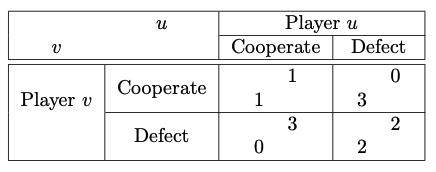
\includegraphics[width=0.8\linewidth]{prisoner.png}
\end{center}

A game requires at least two rational players, and each player can choose from at least two options (strategies). In every possible outcome (strategy profile) each player gets a certain payoff (or cost). The payoff of a player depends on the strategies of the other players. \medskip

A strategy profile is called \textbf{social optimum} (SO) if and only if it minimizes the sum of all costs (or maximizes payoff). \medskip

A strategy is \textbf{dominant} if a player is never worse off by playing this strategy. A dominant strategy profile is a strategy profile in which each player plays a dominant strategy. \medskip

A \textbf{Nash Equilibrium} (NE) is a strategy profile in which no player can improve by unilaterally (the strategies of the other players do not change) changing its strategy. A game can have multiple Nash Equilibria. If every player plays a dominant strategy, then this is by definition a Nash Equilibrium. \medskip

Nash Equilibria and dominant strategy profiles are so called solution concepts. They are used to analyze a game. \medskip

The \textbf{best response} is the best strategy given a belief about the strategy of the other players.


\subsection{Selfish Caching}

Consider computers in a network who want to access a file regularly. Each node $v \in V$ has a demand $d_v$ for the file and wants to minimize the cost for accessing it. To access it, a file can either be cached locally at cost 1 or be requested from another node $u$ with cost $c_{u \to v}$. If we interpret this game as a graph, then the cost $c_{u \to v}$ is equivalent to the length of the shortest path times the demand $d_v$.\medskip

\begin{algorithm}[H]
\caption{Nash Equilibrium for Selfish Mining}
	$S = \{\}$ \\
	\While{$V$ not empty}{
		Let $v$ be the node  maximum demand $d_v$ in $V$\\
		$S = S \cup \{v\}, \; V = V \backslash \{v\}$\\
		Remove every node $u$ from $V$ with $c_{v \to u} \leq 1$
	}
\end{algorithm}
\medskip

Let $NE_−$ denote the Nash Equilibrium with the highest cost (smallest payoff). The Price of Anarchy measures how much a distributed system degrades because of selfish nodes. The Price of Anarchy ($PoA$) is defined as:
$$PoA = \frac{\text{cost}(NE_-)}{\text{cost}(SO)}$$

Let $NE_+$ denote the Nash Equilibrium with the smallest cost (highest payoff). The Optimistic Price of Anarchy ($OPoA$) is defined as:
$$OPoA = \frac{\text{cost}(NE_+)}{\text{cost}(SO)}$$

We have $PoA \geq OPoA \geq 1$. The following shows a network with a Price of Anarchy of $\Theta (n)$

\begin{center}
	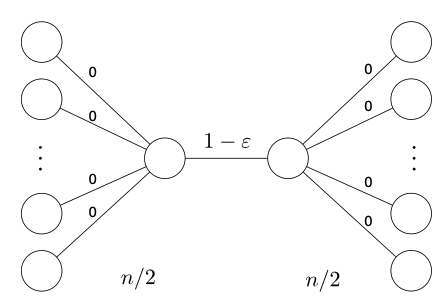
\includegraphics[width=0.7\linewidth]{selfish_caching.png}
\end{center}

The (Optimistic) Price of Anarchy of selfish caching can be $\Theta (n)$.


\subsection{Braess' Paradox}

Consider a game where cars want to travel from $s$ to $t$. Some road's cost depend on the amount of traffic going through them. There are 1000 cars. Adding a super fast road with delay 0 can increase the travel time from $s$ to $t$!
\begin{center}
	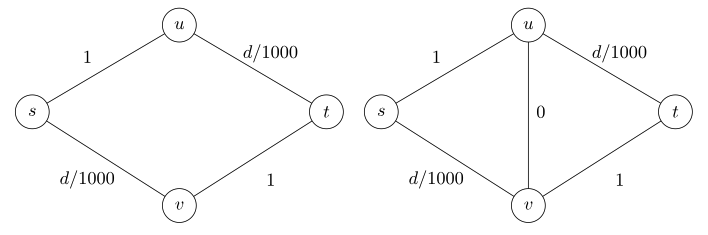
\includegraphics[width=\linewidth]{braess.png}
\end{center}

Each driver acts rationally, thus half of them takes the upper road and half of them the lower. The time for each traveler is then 1 + 500/1000 = 1.5. \medskip

If we introduce the new road with cost 0 between $u$ and $v$, each driver now drives from $s \to v \to u \to t$, leading to a total cost of $2 > 1.5$.


\subsection{Rock-Paper-Scissors}

We will consider the classical game of rock-paper-scissors. No strategy for one player is a Nash Equilibrium: whatever $u$ chooses, $v$ can always switch its strategy s.t. $v$ wins.
\begin{center}
	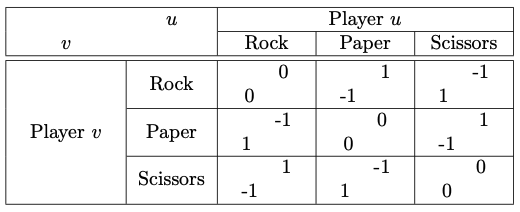
\includegraphics[width=\linewidth]{rps.png}
\end{center}

A \textbf{Mixed Nash Equilibrium} (MNE) is a strategy profile in which at least one player is playing a randomized strategy (choose strategy profiles according to probabilities), and no player can improve their expected payoff by unilaterally changing their (randomized) strategy. Every game has a mixed Nash Equilibrium.\medskip

The Nash Equilibrium of this game is if both players choose each strategy with probability 1/3.


\subsection{Mechanism Design}

Whereas game theory analyzes existing systems, there is a related area that focuses on designing games – mechanism design. The task is to create a game where nodes have an incentive to behave "nicely". \medskip

One good is sold to a group of bidders in an \textbf{auction}. Each bidder $v_i$ has a secret value $z_i$ for the good and tells his bid $b_i$ to the auctioneer. The auctioneer sells the good to one bidder for a price $p$. \medskip

For simplicity, we assume that no two bids are the same, and that $b_1 > b_2 > ...$\medskip

\begin{algorithm}[H]
\caption{First Price Auction}
	Every bidder $v_i$ submits his bid $b_i$\\
	The good is allocated to the highest bidder $v_1$ for the price $b_1 = p$
\end{algorithm}
\medskip

An auction is \textbf{truthful} if no player vi can gain anything by not stating the truth. A First Price Auction is not truthful. \medskip

\begin{algorithm}[H]
\caption{Second Price Auction}
	Every bidder $v_i$ submits his bid $b_i$\\
	The good is allocated to the highest bidder $v_1$ for the price $b_2 = p$
\end{algorithm}
\medskip

Truthful bidding is a dominant strategy in a Second Price Auction. \medskip

We can use this mechanism for selfish caching! We need one node who is first to cache. Every node says for which price it is willing to cache the file. We pay the node with the lowest offer and pay it the second lowest offer to ensure truthful offers. \medskip

Any Nash Equilibrium of Selfish Caching can be implemented for free. \medskip

Mechanism design assumes that the players act rationally and want to maximize their payoff. In real-world distributed systems some players may be not selfish, but actively malicious (byzantine).
